\documentclass{article}

\usepackage{graphicx}
\usepackage{pgfplots}
\usepackage{subcaption}

\title{Text symbol classification using neural networks}
\author{Kacper Ochnik \and Paweł Frankowski}
\date{\today}

\begin{document}

\begin{titlepage}
	\centering
	
\includegraphics[width=0.3\textwidth]{Logo_PK_kolor_EN_PNG.png}\par\vspace{1cm}
	{\textsc{Koszalin University of Technology} \par}
	\vspace{1cm}
	{\Large \textsc{Applications of artificial intelligence project report}\par}
	\vspace{1.5cm}
	{\huge\bfseries Handwritten text symbol recognition with deep neural networks
	\par}
	\vspace{2cm}
	{\Large\itshape {Paweł Frankowski \space Kacper Ochnik}\par}
	\vfill
	supervised by\par
	Dr.~Adam Słowik

	\vfill

	{\large \today\par}
\end{titlepage}

\tableofcontents
\newpage

\section{Introduction}
The significance of digit recognition in the realm of artificial intelligence cannot be overstated, particularly in its application to handwritten digits. This project delves into the intricate process of teaching an AI model to discern and interpret handwritten numerals. With a myriad of potential real-world applications, from automating data entry tasks to enhancing accessibility in digital document processing, the ability of an AI model to accurately recognize handwritten digits holds immense promise. Through the utilization of advanced algorithms and machine learning techniques, this project endeavors to unlock the potential of AI in transforming handwritten digit recognition into a seamless and efficient process.

\newpage
\section{Our goal}

The primary objective of our project is to develop a handwritten text symbol recognition system using deep neural networks. We aimed to create a model capable of accurately identifying and classifying handwritten digits ranging from 0 to 9 on a matrix of 28x28 pixels.

\subsection{Specific objectives}

In pursuit of our overarching goal, we have identified the following specific objectives:

\begin{enumerate}
    \item \textbf{Project setup} - Set up the project environment and install the necessary libraries and packages.
    \item \textbf{Code implementation} - Write Python code to implement the deep neural network architecture. This includes developing modules for data preprocessing, model training, and evaluation.
    \item \textbf{Data Collection} - Gather a comprehensive dataset of handwritten digits (0 to 9) in a 28x28 pixel matrix format from MNIST.
	\item \textbf{Learning} - Train the model using the collected dataset.
	\item \textbf{Optimization} - Improve the model's accuracy through optimization techniques. Accelerate computational efficiency for faster calculations.
    \item \textbf{Testing} - Create testing GUI for the trained model. Evaluate the model's performance metrics.
	\item \textbf{Documentation} - Write a comprehensive report documenting the project's objectives, methodology, and outcomes.
\end{enumerate}

\subsection{Expected Outcomes}

Upon successful completion of our project, we anticipate achieving the following outcomes:

\begin{itemize}
    \item Develop a robust deep neural network model capable of recognizing and classifying handwritten digits from 0 to 9.
    \item Train the model to achieve a acceptable level of accuracy.
\end{itemize}

\newpage
\section{Decision Boundary}

The concept of a decision boundary is fundamental in understanding how a neural network makes predictions and categorizes inputs. In the context of our handwritten text symbol recognition project, the decision boundary plays a crucial role in distinguishing between different handwritten digits.

\subsection{Definition}
A decision boundary is a hypersurface that separates the input space into regions assigned to different classes. In our case, each region corresponds to a specific digit (0 through 9). The decision boundary is learned during the training phase of the neural network and is a reflection of the network's understanding of the features that differentiate one digit from another.

\subsection{Adaptability}
The adaptability of the decision boundary is a key aspect of the neural network's performance. A well-trained model should be capable of adjusting its decision boundary to accommodate variations in handwriting styles, ensuring robust recognition across different writing patterns.

\subsection{Optimization Impact}
During the optimization process, the neural network adjusts its parameters to optimize the decision boundary for accurate classification. Understanding the decision boundary dynamics sheds light on how changes in weights and biases impact the model's ability to discriminate between different digits.

In the subsequent sections, we will delve into the weights and biases optimization process, shedding further light on how these adjustments influence the decision boundary and contribute to the overall performance of our handwritten text symbol recognition system.

\newpage
\section{Weights and Biases}
Weights are indicators of the importance of the input in predicting the final output. Biases are essential as they allow the network to have some flexibility in fitting the data. In the training process of our neural network, the weights and biases play a crucial role in determining the model's performance. Here, we discuss the initialization, calculation, and adjustment of weights and biases in the network. 

\subsection{Initialization}
The \texttt{Layer} class represents a single layer in the neural network. It contains information about the number of nodes in and out, weights, biases, and gradients. The neural network is initialized with random weights using the Xavier/Glorot initialization technique. This method helps in achieving better convergence during training.

\begin{figure}[ht]
    \centering 
    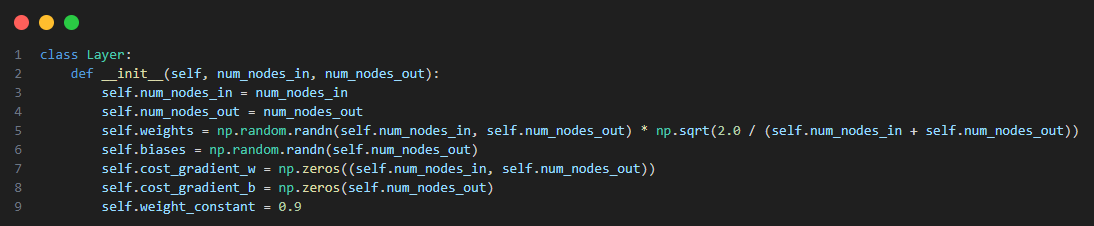
\includegraphics[width=1\textwidth]{images/Xavier-Glorot-initialization-for-weights.png}
    \caption{Initialization of random biases and weights using Xavier/Glorot technique}
    \label{fig:initialized_weights}
\end{figure}

When a neural network is first trained, it is first fed with input. Since it isn't trained yet, we don't know which weights should we use for each input. And so, each input is randomly assigned a weight. It will very likely give incorrect output.

\subsection{Weighted sum of inputs}
In the \texttt{Layer} class, the calculation of outputs begins with the computation of weighted inputs. For each node in the layer, the weighted inputs are calculated using the formula.:
\begin{figure}[ht]
    \centering
    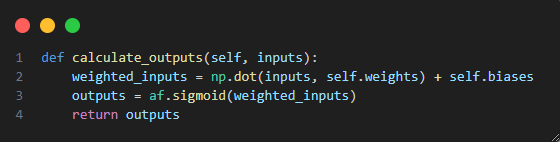
\includegraphics[width=1\textwidth]{images/dot-product-of-inputs-and-weights.png}
    \caption{The dot product of inputs and weights, representing the weighted sum of inputs}
    \label{fig:weighted_sum}
	\subcaption*{The \texttt{calculate outputs} method calculates the dot product of inputs and weights, representing the weighted sum of inputs. The biases are then added to this sum to introduce flexibility in fitting the data. Finally, the result is passed through the sigmoid activation function to introduce non-linearity to the model, and the outputs are obtained.}
\end{figure}

\newpage
\section{Hidden layers}
Proponuje zaminic ten rozdzial na "FFN" (Feedforward Neural Network) i opisac tam jak dziala siec neuronowa, a w tym rozdziale opisac jak wyglada nasz model AI.
...

\newpage
\section{Activation functions}
Activation functions play a crucial role in neural networks, introducing non-linearity to the model and allowing it to learn complex relationships in the data. Here, we describe various activation functions implemented in the \texttt{activation functions} module.

\subsection{Sigmoid function}
The sigmoid function squashes its input to the range (0, 1), making it suitable for binary classification problems.

\begin{equation}
	f(x) = \frac{1}{1 + e^{-x}}
\end{equation}

\begin{equation}
    \begin{tikzpicture}
        \begin{axis}[
            xlabel={$x$},
            ylabel={$f(x)$},
            domain=-5:5,
            samples=100,
            smooth,
            scale=1.5
        ]
            \addplot[blue] {1/(1 + exp(-x))};
            \legend{$f(x) = \frac{1}{1 + e^{-x}}$}
        \end{axis}
    \end{tikzpicture}
\end{equation}

\begin{figure}[ht]
    \centering
    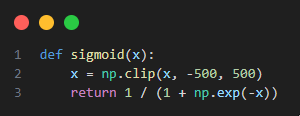
\includegraphics[width=0.5\textwidth]{images/sigmoid-function.png}
    \caption{Sigmoid function}
    \label{fig:sigmoid_function}
	\subcaption*{Limiting the values of x to prevent overflow. Overflow refers to a situation where the exponential function in the sigmoid formula produces very large positive values, causing numerical instability in calculations. The exponential function, especially when dealing with large positive inputs, can lead to floating-point overflow, which means the result becomes too large to be represented within the numerical precision of the system.}
\end{figure}

\subsection{The derivative of the sigmoid function}
The derivative of the sigmoid function is used in the backpropagation algorithm to calculate the gradients of the cost function with respect to the weights and biases. The derivative of the sigmoid function is given by the formula:

\begin{equation}
    f'(x) = f(x) \cdot (1 - f(x))
\end{equation}

\begin{figure}[ht]
    \centering
    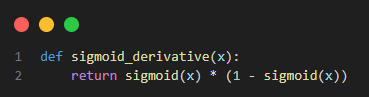
\includegraphics[width=0.5\textwidth]{images/sigmoid-derivative.png}
    \caption{The derivative of the sigmoid function}
    \label{fig:sigmoid_derivativse_function}
\end{figure}

\newpage
\section{Gradient descent and backpropagation}
\subsection{Gradients of the cost function}
\textbf{Gradient Descent} - Is an optimization algorithm that is used to find the weights that minimize the cost function. 
We need two things to do so. Direction in which to navigate and the size of the steps for navigating.
To know which direction to navigate the cost function, gradient descent uses backpropagation. More specifically, it uses the gradients calculated through backpropagation. These gradients are used for determining the direction to navigate to find the minimum point. Descresing slope will lead us to the minimum point.
The cost gradients for weights and biases are initialized with zeros, and during training, these gradients will be updated based on the backpropagation algorithm.

\begin{figure}[ht]
    \centering 
    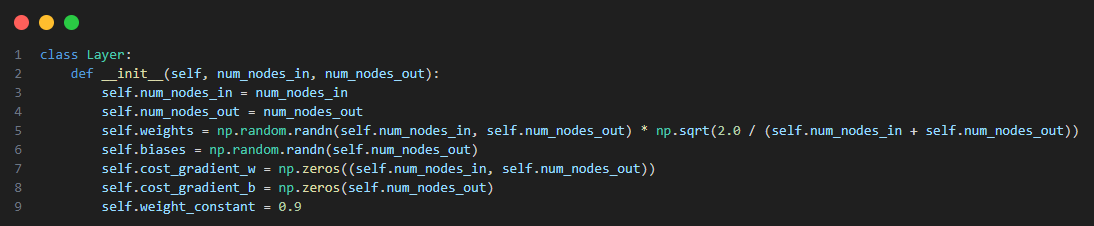
\includegraphics[width=1\textwidth]{images/Xavier-Glorot-initialization-for-weights.png}
    \caption{Initialization a vector of zeros with the same length as the bias vector}
    \label{fig:initialized_cost_gradient}
	\subcaption*{This matrix will be used to accumulate the gradients of the cost function with respect to the weights during the backpropagation process.}
\end{figure}

\begin{figure}[ht]
    \centering 
    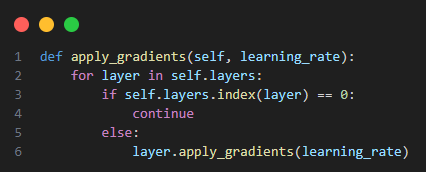
\includegraphics[width=1\textwidth]{images/apply-gradients.png}
    \caption{The \texttt{apply\_gradients} method in \texttt{Neural network} class  updates the weights and biases for each layer.}
    \label{fig:apply_gradients}
\end{figure}

\begin{figure}[ht]
    \centering 
    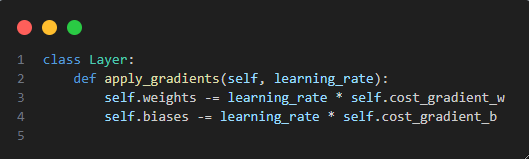
\includegraphics[width=1\textwidth]{images/layer-gradient.png}
    \caption{The \texttt{apply\_gradients} method in \texttt{Layer} class updates the weights and biases for a layer.}
    \label{fig:apply_gradients_on_layer}
    \subcaption*{The \texttt{apply gradients} method is responsible for updating the weights and biases of a layer based on the calculated gradients.}
\end{figure}

\newpage
\subsection{Data loading and learning}

\begin{figure}[ht]
    \centering 
    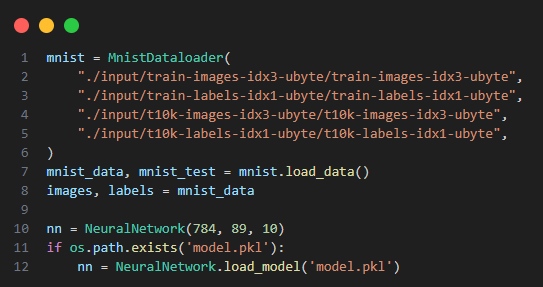
\includegraphics[width=1\textwidth]{images/data-load.png}
    \caption{Data loading from mnist and creating a neural network}
    \label{fig:data_load}
    \subcaption*{A neural network is instantiated with the specified architecture: 784 input nodes, one hidden layer with 89 nodes, and 10 output nodes. Checks if a pre-trained model file \texttt{model.pkl} exists.If it does, the model is loaded from the file. Otherwise, the model is trained using the MNIST dataset.}
\end{figure}

\begin{figure}[ht]
    \centering 
    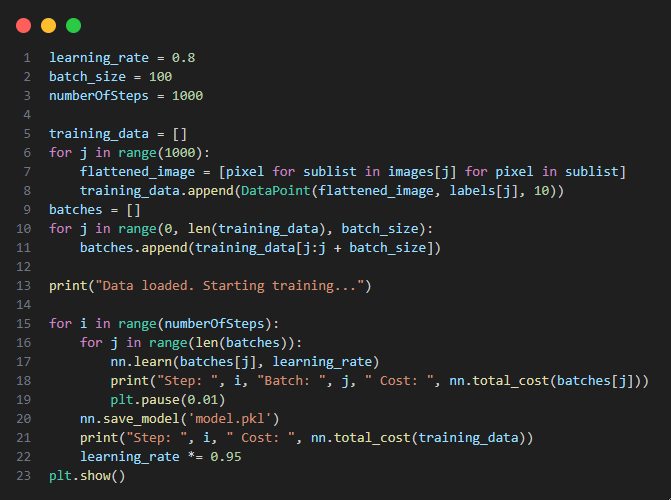
\includegraphics[width=1\textwidth]{images/main.png}
    \caption{Training a neural network using a simple form of gradient descent on the MNIST dataset.}
    \label{fig:learn}
    \subcaption*{\textbf{Learning rate} - determines the step size at each iteration of gradient descent and the speed at which we move down the slope. Learning rate plays important role in between optimization time and accuracy. Step size is measured by a parameter alpha $\alpha$. Small $\alpha$ means small step size, large $\alpha$ means large step size. If its too large then it can jump through minimum of the function. This parameter needs to be optimized. High learning rate results in a higher step value and opposite.\\ \textbf{Batch size} refers to the number of training examples utilized in one iteration. \\ \textbf{The number of steps}, represents the total number of times the entire training dataset is passed forward and backward through the neural network. Too few steps may lead to underfitting, while too many steps may result in overfitting on the training data. The optimal number of steps depends on the complexity of the task and the dataset.}
\end{figure}

\newpage
\subsection{Backpropagation}
\textbf{Backpropagation} - is a training algorithm for feedforward neural networks that propagates the error backward from the output to the input layer.
It plays a crucial role in gradient descent, a process of finding the minimum of the cost function. 
Gradient descent relies on backpropagation to calculate gradients by moving backward in the neural network.
Together, backpropagation and gradient descent is used for the purpose of improving the prediction accuracy of neural networks. 
They help improve prediction accuracy by reducing the output error in neural networks.

\begin{figure}[ht]
    \centering 
    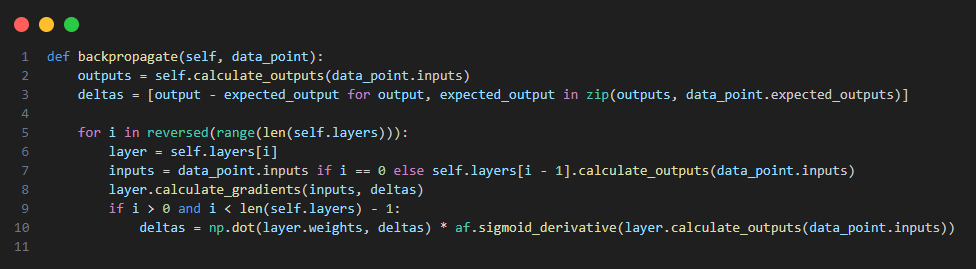
\includegraphics[width=1\textwidth]{images/backpropagate.png}
    \caption{The \texttt{backpropagate} function is part of the neural network training process.}
    \label{fig:backpropagation}
\end{figure}

\begin{figure}[ht]
    \centering 
    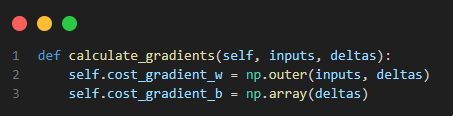
\includegraphics[width=1\textwidth]{images/calculate-gradients.png}
    \caption{The \texttt{calculate\_gradients} method computes the gradients needed for the weight and bias adjustments.}
    \label{fig:calculate_gradients}
    \subcaption*{It represents how much the weights and biases should be changed to minimize the difference between the predicted and expected outputs. It's like figuring out the direction and magnitude of the correction needed to improve the network's performance.}
\end{figure}

\newpage
\section{Cost Landscape}

Understanding the cost landscape is essential for comprehending the optimization process in neural networks. In our project of handwritten text symbol recognition, the cost landscape reflects the relationship between the model's parameters and the cost function, providing insights into the optimization journey.

\subsection{Definition}
The cost landscape, also known as the loss landscape, is a graphical representation of how the cost function varies with changes in the neural network's parameters, such as weights and biases. It visualizes the "landscape" of the optimization problem, showing areas of high and low cost values.

\subsection{Characteristics}
The cost landscape can exhibit various characteristics, including multiple local minima, saddle points, and plateaus. Local minima represent suboptimal solutions, while saddle points pose challenges to gradient-based optimization algorithms. Plateaus, on the other hand, indicate regions of slow convergence, where the optimization process may stagnate.

\subsection{Impact on Optimization}
Navigating the cost landscape effectively is crucial for optimizing the performance of the neural network. Understanding the topology of the landscape helps in selecting appropriate optimization algorithms, setting learning rates, and initializing parameters to avoid getting stuck in local minima or encountering convergence issues.

\subsection{Optimization Strategies}
Based on the insights gained from analyzing the cost landscape, various optimization strategies can be employed to navigate the landscape effectively. Techniques such as stochastic gradient descent, momentum optimization, and adaptive learning rates aim to mitigate the challenges posed by the landscape topology and accelerate convergence towards the global minimum.

In the subsequent sections, we will explore the optimization strategies employed in our project and their impact on improving the performance of our handwritten text symbol recognition system.

\newpage
\section{Learning algorithm - naive approach, calculus approach, digit recognition - Kacper}
Kacper you should check other sections because there could be duplicates!
...

\newpage
\section{Chain rule}
...

\newpage
\section{Testing the network}
...

\newpage
\section{Conclusion}
This is the conclusion of the document.

\end{document}
